
\begin{problem}{Longest Palindromic Subsequence}
    Given a string s, find the longest palindromic subsequence's length in s.

    \footnotetext{LC516}
\end{problem}

\begin{solution}[Recursive]

    As the question ask us to find palindromic subsequence.  The palidromic pattern suggest us to find the recurrance relation involving start \& end of the current string.

    \intution{ let $f(l,r,\_)$ be the length of longest palindromic subsequence for string [l,r]}

    Now, there can be two case: either both are equal or they are not equal.

    \begin{code}
    int findLongestPalindrome(int l, int r, string s1)
    {
        if(l==r)
            return 1;
        if(l>r)
            return 0;
        
        if(s1[l] == s1[r])
            return 2+findLongestPalindrome(l+1,r-1,s1);
        else
        {
            int iLeft = findLongestPalindrome(l+1,r,s1);
            int iRight = findLongestPalindrome(l,r-1,s1);
            return max(iLeft,iRight);
        }
    }
    \end{code}
\end{solution}

\begin{solution}[Iterative]
    This can be achieved by transalation of above recursive.

    Alternative way of thinking the solution is, \rfl{try to build up the solution for lenght1, then lenght2 \dots lengthn}.

    i.e \intution{let dp[i][j] be the maximum lenght substring for string of s[i..j]. Assuming that you already know the answer of subsproblem. Can you express dp[i][j] in terms of lower lenght subsring?}

    \begin{marginfigure}
        
        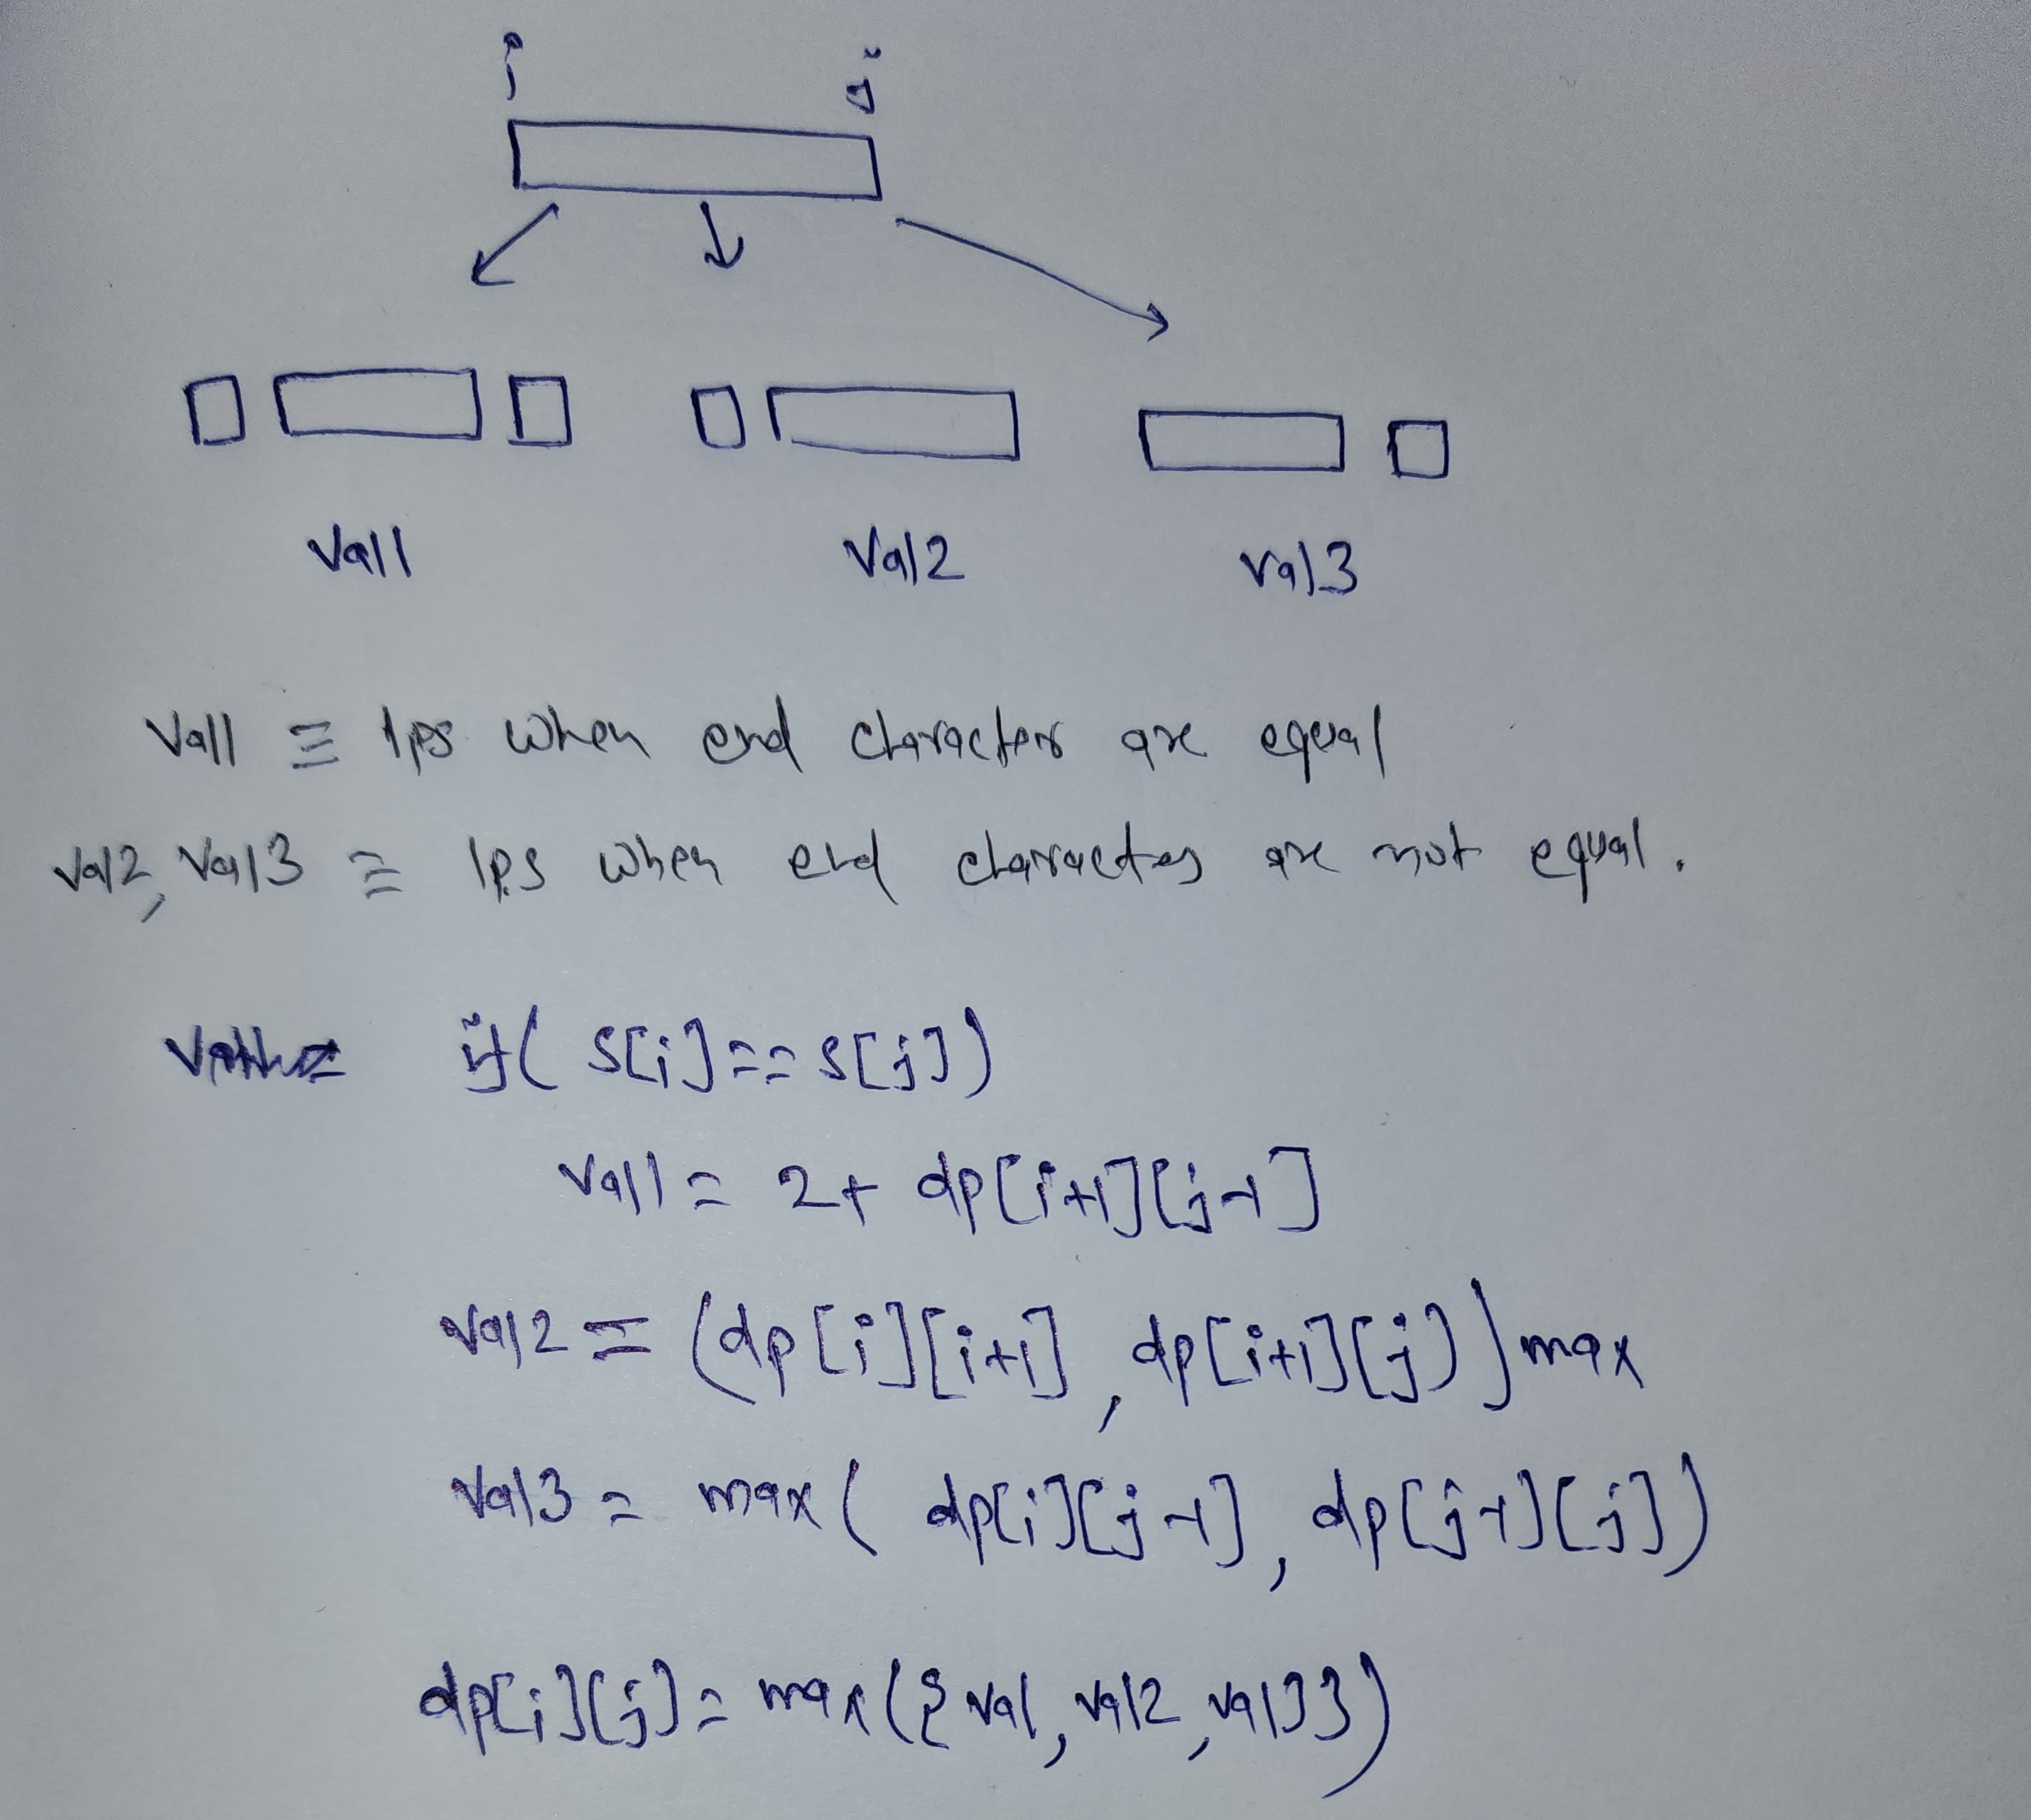
\includegraphics[width=\marginparwidth]{resources/LPS_Division1.jpg}  
    \end{marginfigure}

    \begin{figure}
        \centering
        \caption{Express dp[i][j] in subproblems}
        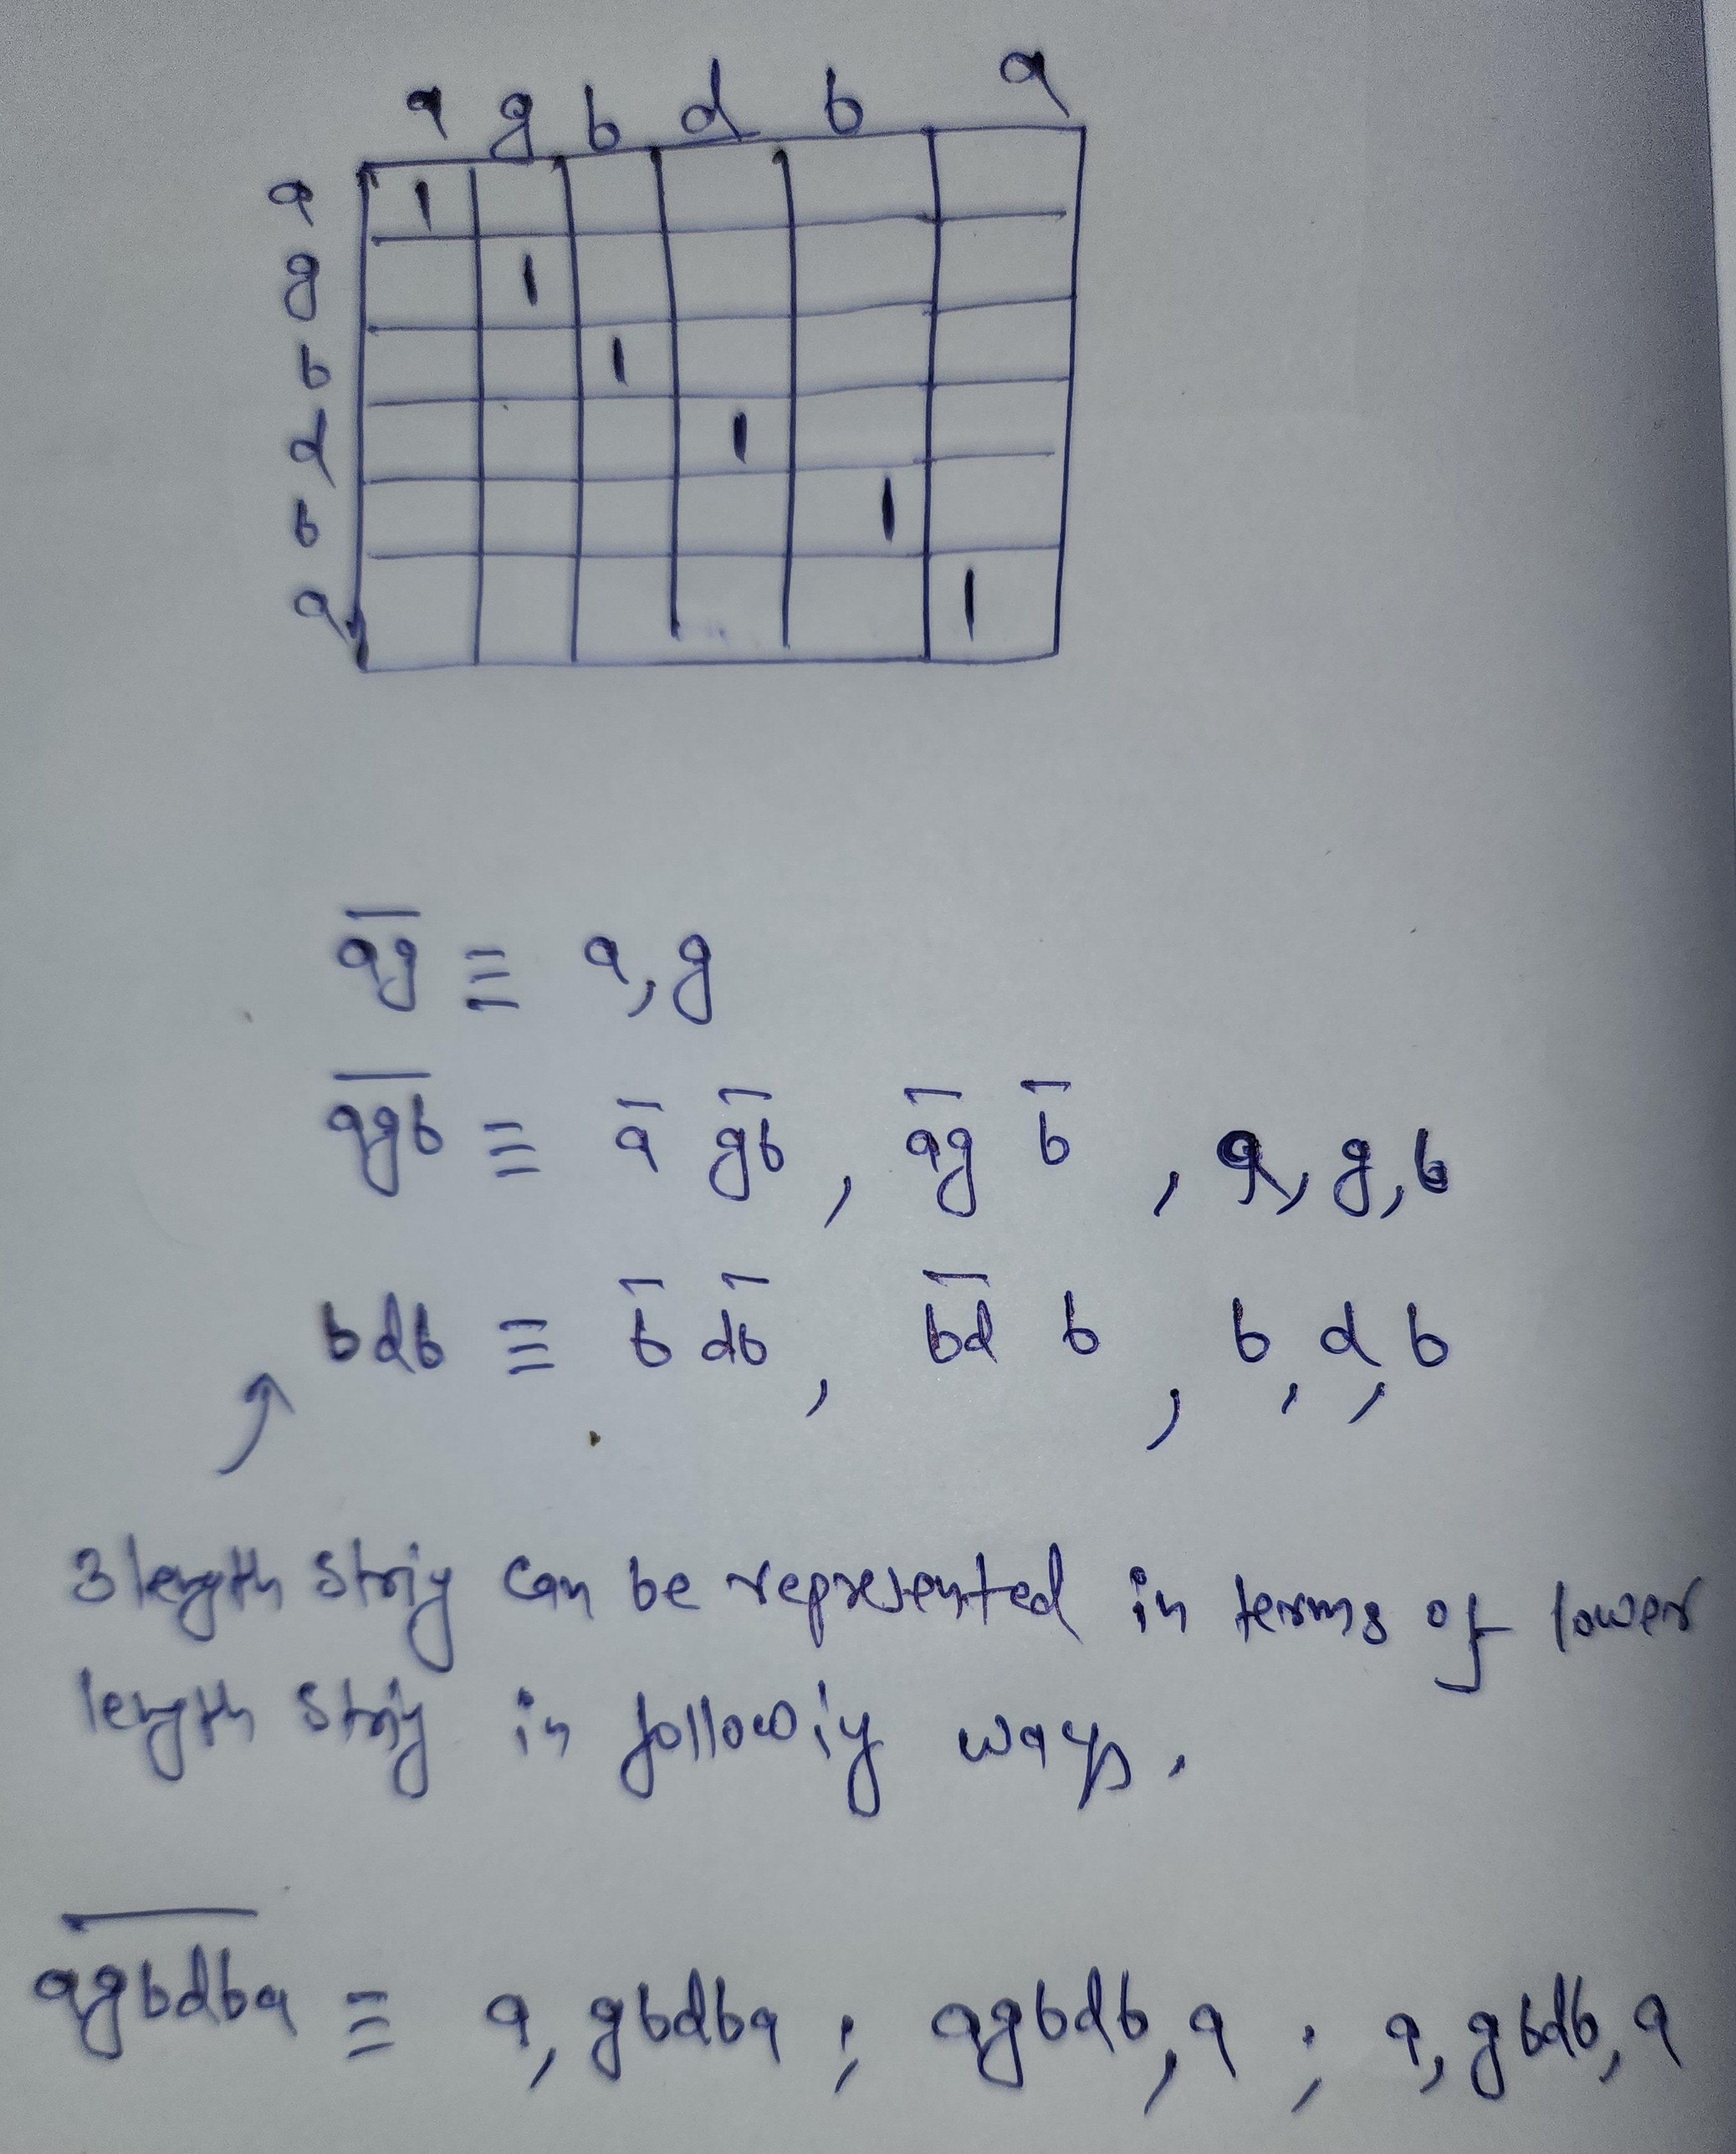
\includegraphics[width=\marginparwidth]{resources/LPS_Division2.jpg} 
    \end{figure}

    \begin{code}
        int longestPalindromeSubsequenceDP(string s1)
        {
            int NRow = s1.length();
            int NCol = s1.length();
        
            vector<vector<int> > dp(NRow,vector<int>(NCol,0));
        
            //Length 1 string is always valid palindrome withlength 1  
            for(int i=0;i<NRow;i++)
                dp[i][i] = 1;
        
            for(int l=2;l<=NRow;l++) //lenght = l
            {
                
                for(int i=0;i<NRow-l+1;i++) 
                {
                    int j = i+l-1; //r-l+1 = interval_size => j-i+1 = l => j = l+1-1
                        
                    int val=0;
                    if(s1[i] == s1[j]) //Recursion Translation
                    {
                        val = 2 + dp[i+1][j-1];
                    }
                    else
                    {
                        int iLeft = dp[i+1][j];
                        int iRight = dp[i][j-1];
                        val = max(iLeft,iRight);
                    }
                    dp[i][j] = val;
                }
            }      
            return dp[0][NCol-1];
        }
    \end{code}

 
    
\end{solution}